\Question{L1}

This question is about LASSO, the $L_1$ norm, and sparsity in general. To recap, sometimes it is desirable to find a solution vector $w$ which has only $k$ non-zero entries, that is, finding a solution that is $k$-sparse. However, solving the problem of:
$$\min L(w)$$
$$s.t. ||w||_0 \leq k$$
Is very computationally difficult because the $L_0$ "norm" is not a true norm and is not a convex function. However, there are many approximations of this problem which are able to be solved quickly, one of them being LASSO where we approximate the $L_0$ term above with the $L_1$ norm.

\begin{Parts}

\Part Before we prove some aspects of the relationship between $L_0$ and $L_1$, let us first get some of the geometric intuition behind this. Consider the follow graph from Wikipedia where the colored lines represent the level-sets of $||w||_p = 1$ for various values of $p$ \\
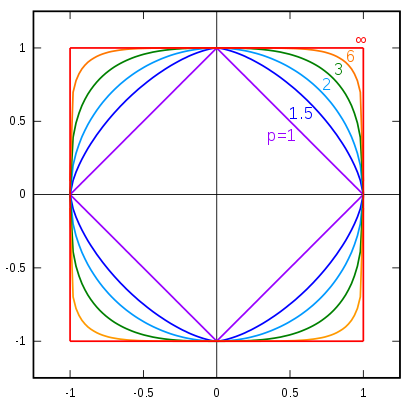
\includegraphics[scale=.5]{src/gs/pic.png}
\\
Draw in the level-set $||w||_0 = 1$ and give an argument why $||w||_1 \leq 1$ is a good convex set approximation and in particular why it is better than any other $L_p$ norm.
\begin{solution}
The $x$ and $y$ axes should be selected (without the origin but this is a minor point)\\
Note that the $L_1$ set is the smallest convex set that contains all points in the $L_0$ set and thus it is the best convex relaxation of the problem to use, at least from the given options. Note that another reason to use $L_1$ is due to the "corner" argument given in lecture.
\end{solution}
\Part The Lasso problem is of the form:  

$$L(w) = \sum_{i=1}^{n} (y_i - w^T x_i)^2 + \lambda \|x \|_1$$
Where the $L_1$ regularization term can be used to encourage feature sparsity. To better understand why $L_1$ regularization leads to sparsity, let us first revisit the concept of the cardinality of $x$, also known as the $L_0$ norm, which is the number of nonzero elements. \\
A non convex loss function that leads to sparsity by penalizing nonzero elements uses the cardinality of $x$:

$$L(w) = \sum_{i=1}^{n} (y_i - w^T x_i)^2 + \lambda \|x \|_0$$ 
In this exercise we will show that $L_1$ regularization is a convex problem which served as a lower bound for the cardinality of $x$.\\

Show that: cardinality$(x) \geq$ $\frac{||x||_1^2}{||x||_2^2}$ \\
Hint: Use the Cauchy-Swartz inequality: $ |x^Ty| \leq \|x\|_2 \|y\|_2$ for x being the nonzero elements of vector x and y a vector that you will determine. \\
\\\indent \\
\begin{solution}
If we set y = sign(x) this will lead to: \\ 
$ \| x \|_1 \leq \|x\|_2 \sqrt{n}$ where n = cardinality of x \\
This leads to the lower bound: \\
cardinality(x) $\geq$ $\frac{||x||_1^2}{||x||_2^2}$ \\
\\\indent
Note: If we project x onto subspace with directions i where $x_i \neq 0$ then the resulting vector z will be of size card(x) or the number of nonzero values of x. 
Since the only $x_{is}$ that are not in z are equal to zero, this implies that $\lVert x\rVert_2 = \lVert z\rVert_2$ and  $\lVert x\rVert_1 = \lVert z\rVert_1$ \\ \\
\end{solution}
 
\Part What does bounding the cardinality of x by the L1 norm tell us about L1 regularization for feature selection?

\end{Parts}

\newpage
